\section{字体篇}
%
%
%\begin{faq}{LaTeX字体是如何处理的}
%
%LaTeX 2ε目前的字体机制称为``新字体选择机制''(New Font Selection
%Scheme,NFSS)。它将文本字体分为五个互不干扰的属性(数学字体初学者不必过早了解):
%\begin{enumerate}
%  \item
%  
%编码(encoding)。这个属性初学者暂时不必了解。在(pdf)latex和uplatex中,默认的西文编码称为OT1;在xelatex中,默认的编码称为EU2,就是Unicode。
%  \item
%  字族(family)。一套成风格的字型的统称,如cmr、ptm(times)等。\LaTeXe{}
%  预先定义了三个切换字族的命令:\cs{rmfamily}(衬线体)、\cs{sffamily}(无衬线体)、\cs{ttfamily}(等宽体)。
%  \item
%  
%系列(series)。在一般的字体中一般表示字重(weight)。如粗体命令为\cs{bfseries},正常粗细为\cs{mdseries}。
%  \item
%  
%字形(shape)。在同一字族、同一系列下的风格差异,如斜体\cs{slshape}、意大利斜体\cs{itshape}、正体\cs{upshape}、小型大写\cs{scshape}。
%  \item
%  字号(size)。以上四种变化是字型(typeface)的变化,而这是同一字型下不同大小的变化。LaTeX
%  2ε提供了成套的字号命令,如\cs{normalsize}、\cs{small}、\cs{scriptsize} 等。
%\end{enumerate}
%
%中文字体的方面,不同的中文解决方案的处理也有不同,这里就不介绍了。
%\end{faq}
%
%
%\begin{faq}{获取位图字体}
%\end{faq}
%
%
%\begin{faq}{PDF格式图片插入过程中的字形缺失}
%\end{faq}
%
%
%\begin{faq}{为数学排版选择Type
%  1字体}
%\end{faq}
%
%
%\begin{faq}{Type 1字体配置}
%\end{faq}
%
%
%\begin{faq}{切换到T1时字体变得模糊}
%\end{faq}
%
%
%\begin{faq}{由于Ghostscript太旧造成字体模糊}
%\end{faq}
%
%
%\begin{faq}{如何使用斜体}
%
%斜体一般是西文字体用的,在中文中不用斜体。
%
%斜体这个名字比较误导,因为它对应英文的两个名字:倾斜体(slanted,指字形风格大致相同但是倾斜)和意大利体(italic,指字形设计为接近手写的形态,同时也就出现了倾斜)。
%
%两种情况下分别有 \cs{slshape} 和 \cs{itshape} 两个命令,使用例如
%\verb|{\slshape slanted}| 及\verb|{\itshape 
%italic}|;也有把斜体内容作为参数的命令(推荐使用这种),如\textsl{slanted}及\textit{italic}。
%\end{faq}
%
%
%\begin{faq}{如何使用粗体}
%
%\begin{enumerate}
%  \def\labelenumi{\arabic{enumi}.}
%  \item
%  \cs{mathbf}
%  
%  \cs{mathbf}
%  会将数学模式取消再来取用字型,因此它加粗的不是数学符号,而是公式里的一般文字。\cs{mathbf} 
%  只能在公式内部使用:
%\end{enumerate}
%
%\begin{verbatim}
%\documentclass{article}
%\begin{document}
%$\mathbf{equation: f(x,y) = \alpha x^2 + \beta y^2}$
%\end{document}
%\end{verbatim}
%
%效果如下:
%% \includegraphics{https://images-cdn.shimo.im/tmTzWYcpaSUPPQCQ/image.png!thumbnail}
%
%\begin{enumerate}
%  \def\labelenumi{\arabic{enumi}.}
%  \setcounter{enumi}{1}
%  \item
%  \cs{boldmath}
%  
%  \cs{boldmath} 可以将整套数学字体切换为粗体版本,这个命令只能在公式外使用:
%\end{enumerate}
%
%\begin{verbatim}
%\documentclass{article}
%\begin{document}
%\boldmath{$f(x,y) = \alpha x^2 + \beta y^2$}
%\end{document}
%\end{verbatim}
%
%效果如下:
%% \includegraphics{https://images-cdn.shimo.im/FT1utRInpn8FWCZX/image.png!thumbnail}
%
%\begin{enumerate}
%  \def\labelenumi{\arabic{enumi}.}
%  \setcounter{enumi}{2}
%  \item
%  \cs{boldsymbol}
%  
%  amsmath 提供了一个 \cs{boldsymbol} 命令(由调用的 amsbsy
%  宏包提供),用于打破 \cs{boldmath}
%  的限制,在公式内部将一部分符号切换为粗体:
%\end{enumerate}
%
%\begin{verbatim}
%\documentclass{article}
%\usepackage{amsbsy}%或者直接调用常用宏包amsmath
%\begin{document}
%$f(x,y) = \boldsymbol{\alpha x^2 + \beta y^2}$
%\end{document}
%\end{verbatim}
%
%效果如下:
%% \includegraphics{https://images-cdn.shimo.im/FiwJiO2EZeYTf4j7/image.png!thumbnail}
%
%\begin{enumerate}
%  \def\labelenumi{\arabic{enumi}.}
%  \setcounter{enumi}{3}
%  \item
%  \cs{bm}
%\end{enumerate}
%
%\begin{verbatim}
%\documentclass{article}
%\usepackage{bm}
%\begin{document}
%$\sum x_i y_i$,
%$\bm{\sum x_i y_i}$,
%${\bm \sum}{\bm x_i}{\bm y_i}$.
%\end{document}
%\end{verbatim}
%
%效果如下:
%% \includegraphics{https://images-cdn.shimo.im/yKpDot5b9oUc6ww3/image.png!thumbnail}
%
%\begin{enumerate}
%  \def\labelenumi{\arabic{enumi}.}
%  \setcounter{enumi}{4}
%  \item
%  \cs{pmb}
%  
%  需使用 amamath 宏包。
%  \item
%  \textbf
%  文本加粗
%\end{enumerate}
%
%\begin{verbatim}
%\documentclass{article}
%\begin{document}
%\textbf{equation: $f(x,y)=\alpha x^2+\beta y^2$}
%\end{document}
%\end{verbatim}
%
%效果如下:
%% \includegraphics{https://images-cdn.shimo.im/ZFmJXLZAIGQKq0VQ/image.png!thumbnail}
%
%\begin{enumerate}
%  \def\labelenumi{\arabic{enumi}.}
%  \setcounter{enumi}{6}
%  
%  \item
%  \cs{bfseries}
%  \cs{bfseries} 影响之后所有的字符,如果想让它在局部生效,需使用花括号分组:
%\end{enumerate}
%
%\begin{verbatim}
%\documentclass{article}
%\begin{document}
%{\bfseries equation: $f(x,y) = \alpha x^2 + \beta y^2$}\\
%equation: $f(x,y) = \alpha x^2 + \beta y^2$.\\
%\bfseries equation: $f(x,y) = \alpha x^2 + \beta y^2$\\
%equation: $f(x,y) = \alpha x^2 + \beta y^2$.\\
%\end{document}
%\end{verbatim}
%
%效果如下:
%% \includegraphics{https://images-cdn.shimo.im/rafHmr9a7JYYebWs/image.png!thumbnail}
%参考: Ishort-zh-cn LaTeX入门,刘海洋。
%\url{http://blog.sina.com.cn/s/blog_5e16f1770100nqwx.html}
%\end{faq}
%
%
%\begin{faq}{如何设置文档字体为本机已安装字体?}
%\end{faq}
%
%
%\begin{faq}{如何通过字体文件名来调用未安装本机字体?}
%\end{faq}
%
%
%\begin{faq}{字体大小经常出现警告,该引用什么宏包解决?}
%\end{faq}
%
%
%\begin{faq}{有些特殊文字怎么加入Latex文档,例如symbol\{"ff0e\}编译后为空白}
%\end{faq}
%
%
%\begin{faq}{如何查看字体和行间距,然后怎样修改}
%\end{faq}
%
%
%\begin{faq}{字体相对大小指令}
%
%\cs{small} 等命令对应的字体大小与文章 \cs{documentlcass} 中指定的字体有关,对应
%10, 11, 12pt 三种全局字体大小的情况如下表所示, 指令 10pt 11pt 12pt
%% \tiny                           5 6 6
%% \scriptsize                 7 8 8
%% \footnotesize            8 9 10
%% \small                        9 10 10.95
%% \normalsize              10 10.95 12
%% \large                       12 12 14.4
%% \Large                      14.4 14.4 17.28
%% \LARGE                    17.28 17.28 20.74
%% \huge                       20.74 20.74 24.88
%% \Huge                      24.88 24.88 24.88
%\end{faq}
%
%
%\begin{faq}{在latex公式中如何将某一个字母或者希腊符号设置成某一个字体?}
%\end{faq}
%
%
%
